\documentclass{article}

\IfFileExists{iclr2026_conference.sty}
  {\usepackage{iclr2026_conference,times}}
  {\usepackage{times}}

\usepackage{microtype}
\usepackage{amsmath,amssymb}
\usepackage{array}
\usepackage{booktabs}
\usepackage{xcolor}
\usepackage{graphicx}
\usepackage{tikz}
\usetikzlibrary{arrows.meta,calc,fit,positioning}
\usepackage[colorlinks=true,linkcolor=blue,citecolor=blue,urlcolor=blue]{hyperref}

\title{Evolve}
\author{Anonymous Authors}
\date{}

\newcommand{\Dset}{\mathcal{D}}
\newcommand{\Mem}{\mathcal{M}}
\newcommand{\Tree}[1]{\mathcal{T}(#1)}
\newcommand{\valid}{\mathrm{valid}}
\newcommand{\sg}{\operatorname{sg}}

\definecolor{searchblue}{HTML}{4C6FA8}
\definecolor{memorygreen}{HTML}{4F806A}
\definecolor{policyteal}{HTML}{3F7F82}
\definecolor{verifyred}{HTML}{8B4B4B}
\definecolor{softgray}{HTML}{F1F3F5}
\definecolor{linegray}{HTML}{4F5963}
\definecolor{statefill}{HTML}{F1F5FA}
\definecolor{stateborder}{HTML}{B8C7D9}
\definecolor{memoryfill}{HTML}{EDF5F0}
\definecolor{neutralfill}{HTML}{ECEFF2}
\definecolor{rlfill}{HTML}{F8EEEE}

\begin{document}

\maketitle

\section{Preliminaries}
\label{secpreliminaries}

A discovery problem $d$ specifies a candidate space, validity constraints, a transition rule, and an evaluator. The initial archive contains at least one valid baseline. Starting from a retained parent $p$, the policy generates a response $y$ and the transition rule constructs a candidate $s=T_d(p,y)$. The evaluator returns a scalar reward $r=R_d(s)$ and textual feedback $f=F_d(s)$. The feedback may contain a failed test, an execution error, a violated constraint, or a numerical diagnostic. Invalid candidates receive the task failure reward and are not eligible to become future parents.

Scientific discovery is evaluated by the strongest valid result found within a finite evaluation budget. Let $\Pi$ denote the complete adaptive search procedure and let $B$ be its total number of evaluations. Its objective is
\begin{equation}
J_B(\Pi)
=
\mathbb{E}_{s_1,\ldots,s_B\sim\Pi}
\left[
\max_{\substack{1\leq i\leq B\\s_i\ \valid}}
R_d(s_i)
\right].
\label{eqobjective}
\end{equation}
This objective differs from expected reward maximization. A direction that usually fails but occasionally produces an exceptional candidate can be preferable to a reliable direction whose outcomes are only moderate. The search and learning signals below are therefore designed to preserve and increase upper tail outcomes.
Every retained valid candidate is a node in a rooted tree. An edge records that a child was generated by modifying its parent. The tree preserves local descent paths and the flat archive $\Dset_t$ lets candidates from different branches compete globally. Failed candidates are not inserted as future parents, but their rewards and diagnostics remain training evidence. The output after step $t$ is the best valid archived candidate $s_t^*=\operatorname*{arg\,max}_{s\in\Dset_t}R_d(s)$. Keeping this archive makes discovery monotone in the sense that a later policy update cannot erase an earlier best result.

\section{Framework}
\label{secframework}

The framework couples max oriented tree search, causal memory, and online policy optimization in one closed loop. At each step, the search rule selects a diverse set of parents from the archive. The fixed rollout budget for each parent is divided among a selected memory prompt, a no memory control, and an exploratory memory prompt. A single language model samples all candidates. The verifier evaluates every candidate and returns reward and feedback. Valid candidates expand the tree, all outcomes train the policy, and matched outcomes determine which lessons remain useful. Figure~\ref{figframework} shows this information flow.

\begin{figure}[t]
\centering
\resizebox{\linewidth}{!}{%
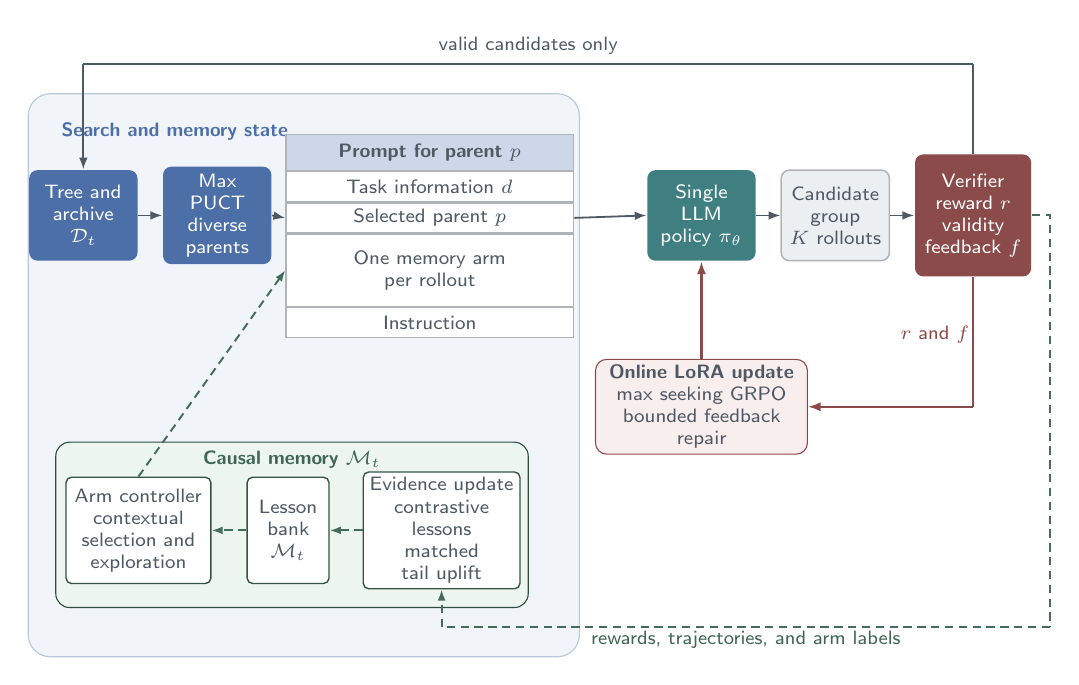
\begin{tikzpicture}[
  x=1cm,
  y=1cm,
  font=\sffamily\footnotesize,
  anchorbox/.style={rounded corners=3pt, align=center, text=white,
    text width=1.20cm, minimum height=1.15cm, inner sep=2.5pt,
    font=\sffamily\scriptsize, line width=0.55pt},
  data/.style={rounded corners=3pt, draw=linegray!45, fill=neutralfill,
    align=center, text=linegray, text width=1.20cm, minimum height=1.15cm,
    inner sep=2.5pt, font=\sffamily\scriptsize, line width=0.55pt},
  promptrow/.style={draw=linegray!45, fill=white, text=linegray,
    text width=3.55cm, minimum height=0.38cm, align=center,
    inner sep=1.5pt, font=\sffamily\scriptsize, line width=0.45pt},
  memcell/.style={rounded corners=2pt, draw=memorygreen!65!black,
    fill=white, text=linegray, minimum height=1.35cm, align=center,
    inner sep=2pt, font=\sffamily\scriptsize, line width=0.5pt},
  flow/.style={-{Latex[length=1.5mm,width=1.1mm]}, draw=linegray, line width=0.65pt},
  evidence/.style={-{Latex[length=1.4mm,width=1.0mm]}, draw=memorygreen!85!black, densely dashed, line width=0.7pt},
  learn/.style={-{Latex[length=1.6mm,width=1.15mm]}, draw=verifyred, line width=0.75pt}
]

% Search and memory state
\node[draw=stateborder, fill=statefill, rounded corners=8pt,
      minimum width=7.00cm, minimum height=7.15cm] (state) at (3.35,2.15) {};
\node[anchor=north west, font=\sffamily\scriptsize\bfseries, text=searchblue]
      at (0.15,5.48) {Search and memory state};

% Prompt card
\node[promptrow, fill=searchblue!28, text=linegray, minimum height=0.46cm,
      font=\sffamily\scriptsize\bfseries] (ph) at (4.95,4.98)
      {Prompt for parent $p$};
\node[promptrow, below=0pt of ph] (p1) {Task information $d$};
\node[promptrow, below=0pt of p1] (p2) {Selected parent $p$};
\node[promptrow, below=0pt of p2, minimum height=0.92cm] (p3)
      {One memory arm \\per rollout\\[-2pt]
       \tiny
       };
\node[promptrow, below=0pt of p3] (p5) {Instruction}
;
% Main generation path
\node[anchorbox, fill=searchblue] (archive) at (0.55,4.18)
      {Tree and archive\\$\Dset_t$};
\node[anchorbox, fill=searchblue] (select) at (2.25,4.18)
      {Max PUCT\\diverse parents};
\node[anchorbox, fill=policyteal] (policy) at (8.40,4.18)
      {Single LLM\\policy $\pi_\theta$};
\node[data] (candidates) at (10.10,4.18)
      {Candidate group\\$K$ rollouts};
\node[anchorbox, fill=verifyred, text width=1.30cm, minimum height=1.55cm]
      (verifier) at (11.85,4.18)
      {Verifier\\reward $r$\\validity\\feedback $f$};

\draw[flow] (archive.east) -- (select.west);
\draw[flow] (select.east) -- (p2.west);
\draw[flow] (p2.east) -- (policy.west);
\draw[flow] (policy.east) -- (candidates.west);
\draw[flow] (candidates.east) -- (verifier.west);

% Valid candidates return to search
\coordinate (validright) at (11.85,6.10);
\coordinate (validleft) at (0.55,6.10);
\draw[draw=linegray, line width=0.65pt] (verifier.north) -- (validright);
\draw[draw=linegray, line width=0.65pt] (validright) -- (validleft)
      node[midway, above, font=\sffamily\scriptsize, text=linegray]
      {valid candidates only};
\draw[flow] (validleft) -- (archive.north);

% Causal memory with three internal cells
\node[draw=memorygreen!60!black, fill=memoryfill, rounded corners=5pt,
      minimum width=6.00cm, minimum height=2.10cm] (membg) at (3.20,0.25) {};
\node[font=\sffamily\scriptsize\bfseries, text=memorygreen!80!black]
      at (3.20,1.08) {Causal memory $\Mem_t$};
\node[memcell, text width=1.70cm] (controller) at (1.25,0.18)
      {Arm controller\\contextual\\selection and\\exploration};
\node[memcell, text width=0.90cm] (bank) at (3.15,0.18)
      {Lesson bank\\$\Mem_t$};
\node[memcell, text width=1.85cm] (evidence) at (5.10,0.18)
      {Evidence update\\contrastive lessons\\matched tail uplift};
\draw[evidence] (evidence.west) -- (bank.east);
\draw[evidence] (bank.west) -- (controller.east);
\draw[evidence] (controller.north) -- (p3.west);

% Arm tagged evidence returns below every component
\coordinate (memouter) at ($(verifier.east)+(0.23,0)$);
\coordinate (memlowleft) at (5.10,-1.05);
\coordinate (memlowright) at (memouter |- memlowleft);
\draw[draw=memorygreen!85!black, densely dashed, line width=0.7pt]
      (verifier.east) -- (memouter) -- (memlowright);
\draw[evidence] (memlowright) --
      node[midway, below, fill=white, inner sep=1pt,
           font=\sffamily\scriptsize, text=memorygreen!80!black]
      {rewards, trajectories, and arm labels}
      (memlowleft) -- (evidence.south);

% Online policy update in a separate lane
\node[draw=verifyred, fill=rlfill, rounded corners=4pt, text=linegray,
      text width=2.55cm, minimum height=1.12cm, align=center,
      inner sep=2pt, font=\sffamily\scriptsize] (update) at (8.40,1.75)
      {\textbf{Online LoRA update}\\max seeking GRPO\\bounded feedback\\repair};
\coordinate (rlturn) at (verifier.south |- update.east);
\draw[draw=verifyred, line width=0.75pt] (verifier.south) -- (rlturn)
      node[pos=0.44, left, fill=white, inner sep=1pt,
           font=\sffamily\scriptsize, text=verifyred] {$r$ and $f$};
\draw[learn] (rlturn) -- (update.east);
\draw[learn] (update.north) -- (policy.south);
\end{tikzpicture}
}%
\caption{Closed loop discovery.}
\label{figframework}
\end{figure}

\subsection{Max Oriented Tree Search}
\label{secsearch}

The search rule treats every archived state as a possible parent. At step $t$, state $s$ receives
\begin{equation}
\operatorname{Score}_t(s)
=
Q_t(s)
+c\,\Delta_t P_t(s)
\frac{\sqrt{1+T_t}}{1+n_t(s)}.
\label{eqpuct}
\end{equation}
Here $Q_t(s)$ is the best reward among children generated directly from $s$, with $R_d(s)$ used before the first expansion. The quantity $T_t$ is the total rollout effort so far and $n_t(s)$ counts effort assigned to $s$ or any descendant of $s$. The scale $\Delta_t$ is the observed reward range with a small positive floor. It puts exploration on the same reward scale as exploitation and remains defined when all archived rewards agree.
The prior depends only on archive rank. If $\rho_t(s)$ is the reward rank with rank one assigned to the best of $N_t$ states, then
\begin{equation}
P_t(s)
=
\frac{N_t-\rho_t(s)+1}{\sum_{j=1}^{N_t}j}.
\label{eqrankprior}
\end{equation}
Ranks keep one reward outlier or an arbitrary task scale from absorbing nearly all prior mass. Every retained state still receives nonzero exploration probability. The exploitation term uses a maximum because averaging a rare discovery with several failed children would hide the event that determines Eq.~\eqref{eqobjective}. The lineage count prevents a successful family from receiving unlimited budget merely because its best observed reward remains high.
Selecting the highest scores independently can fill a batch with nearly identical relatives. Once a parent is selected, its ancestors and descendants are blocked for the rest of that batch. If blocking leaves too few parents, the remaining positions are filled by score. After evaluation, exact duplicates are removed, each parent keeps its strongest children, and the archive retains high reward candidates together with the roots. These controls preserve several search basins without changing the best so far objective.

\subsection{Causal Memory}
\label{secmemory}

Memory is treated as an intervention rather than as text that is presumed useful. Naive retrieval creates a self reinforcing loop. An early lesson can arise from a stochastic success, shift later proposals toward similar candidates, and then receive more apparent confirmation because it is shown more often. Retrieval frequency is then confused with improvement. Diversity falls and alternative basins lose the trials needed to challenge the current strategy. A second bias arises when prompt variants receive unequal sample counts, since the expected maximum increases with the number of samples even when their underlying reward distributions are identical.

The memory maker extracts concise lessons by contrasting each child with its parent and by contrasting successful attempts with failures. The parent comparison identifies which change produced an outcome instead of restating an already strong construction. Failures are sampled across distinct diagnostic signatures so one frequent error cannot dominate extraction. Lessons describe transferable operations or failure avoidance rules. Solution level constructions and over specific code are rejected because copying a complete construction can fix the global search pattern and collapse subsequent generations into one basin. Near duplicates are consolidated in the memory bank $\Mem_t$.

For each selected parent $p$, the model reads a compact lesson catalog and chooses a small relevant set or chooses no lesson. The existing group of $K$ rollouts is then divided among a selected lesson arm, a no memory arm, and an arm containing an under tested lesson. Their counts obey $K_{\mathrm{sel}}+K_0+K_{\mathrm{exp}}=K$. This design is budget neutral. All rollouts remain in the same group for policy learning, while their arm identities are retained for memory credit. Outcome credit uses one lesson per tested arm when lesson level attribution is required.

Memory is credited by matched tail uplift. Let $\mathbf r_a$ and $\mathbf r_0$ contain rewards from a memory arm and its no memory control under the same parent and policy snapshot. Set $n=\min(K_a,K_0)$. For sorted rewards $r_{(1)}\leq\cdots\leq r_{(K)}$, the expected maximum of a uniformly selected size $n$ subset is
\begin{equation}
\widehat M_n(\mathbf r)
=
\sum_{j=n}^{K}
\frac{\binom{j-1}{n-1}}{\binom{K}{n}}
r_{(j)}.
\label{eqsubsamplemax}
\end{equation}
The estimated effect is $\widehat\Delta_a=\widehat M_n(\mathbf r_a)-\widehat M_n(\mathbf r_0)$. Both terms are now best of $n$, so an arm cannot earn credit merely by receiving more samples. Matching the parent, policy snapshot, and search step removes the main contextual confounders. The causal interpretation assumes comparable rollout randomness and no interaction among arms during the matched evaluation. When an arm contains several lessons, the effect belongs to that set rather than to an individual lesson.

An under tested lesson receives trials through the upper confidence score
\begin{equation}
\operatorname{UCB}_t(\ell)
=
\overline{\Delta}_\ell
+c_m s_t
\sqrt{\frac{\log(1+N_t)}{N_\ell}},
\label{equcb}
\end{equation}
where $\overline{\Delta}_\ell$ is its mean matched uplift, $N_\ell$ is its number of controlled trials, $N_t$ is the total amount of memory evidence, and $s_t$ is the observed uplift scale. The score applies after a lesson has been tested, while an untested lesson receives priority. The uncertainty bonus gives neglected lessons a controlled route back into the search. Retention is driven primarily by matched uplift, while validity and improvement over the parent remain diagnostics. The no memory arm is kept throughout training because without it, changes in parent quality, policy parameters, and task difficulty would be indistinguishable from the effect of memory.

\subsection{Max Seeking Online Reinforcement Learning}
\label{secrl}

The proposal model is adapted online through LoRA. Rollouts produced from the same parent are pooled into one group even when they came from different memory arms. For a parent $p$, the risk seeking objective is
\begin{equation}
\mathcal J_\beta(\pi\mid p)
=
\frac{1}{\beta}
\log
\mathbb E_{y\sim\pi(\cdot\mid p)}
\left[\exp\!\left(\beta R_d(y)\right)\right],
\qquad \beta>0.
\label{eqentropicobjective}
\end{equation}
It approaches expected reward as $\beta$ approaches zero and the attainable upper reward as $\beta$ grows. For a sampled group of $K$ responses, the tilted mass is $q_\beta(i)=\exp(\beta r_i)/\sum_j\exp(\beta r_j)$. The concentration is chosen separately for each group by solving $D_{\mathrm{KL}}(q_\beta\Vert U_K)=\gamma$, where $U_K$ is uniform and $0<\gamma<\log K$. Fixing this information distance makes selection pressure invariant to reward shifts and positive rescaling because $\beta$ adapts to the observed reward spread. If ties make the target concentration unattainable, the most concentrated available tilt is used.

Each response is compared with a normalizer built from its siblings. With $r_{\max}=\max_j r_j$, the leave one out advantage is
\begin{equation}
Z_{-i}
=
\frac{1}{K-1}
\sum_{j\ne i}
\exp\!\left(\beta(r_j-r_{\max})\right),
\qquad
A_i^{\max}
=
\frac{\exp\!\left(\beta(r_i-r_{\max})\right)}{Z_{-i}}-1.
\label{eqmaxadvantage}
\end{equation}
This group relative signal assigns most policy gradient mass to the upper tail without learning a value model. It is zero when all sibling rewards are equal because the scalar evaluator has supplied no evidence that one response is preferable. Standard mean centered optimization would instead favor typical reward and can suppress rare high value responses that determine Eq.~\eqref{eqobjective}.

Verifier feedback supplies the missing repair signal on failed responses. Let $\pi_{\bar\theta}$ be the frozen rollout policy and let $q_{\bar\theta}$ be the same policy evaluated after the diagnostic $f_i$ is added to the context. For token $y_{i,l}$, define
\begin{equation}
A^{\mathrm{fb}}_{i,l}
=
\log q_{\bar\theta}
\left(y_{i,l}\mid p,f_i,y_{i,<l}\right)
-
\log \pi_{\bar\theta}
\left(y_{i,l}\mid p,y_{i,<l}\right).
\label{eqfeedbackadvantage}
\end{equation}
The model parameters are identical in both terms, so the detached log ratio isolates how the diagnostic changes the model assessment of each sampled token. A negative value discourages a token that becomes less plausible after the error is revealed. A positive value preserves a token that remains compatible with repair. This gives dense credit when several failures share the same scalar reward and the group reward advantage has collapsed to zero.

With failure indicator $d_i$, the combined token advantage is $A_{i,l}=A_i^{\max}+\lambda_f d_i A^{\mathrm{fb}}_{i,l}$. The coefficient is controlled by the observed validity deficit. It has full strength below a lower validity threshold, decreases linearly between the lower threshold and a target validity rate, and becomes zero once the target is reached. The token signal is clipped and its mean magnitude is bounded relative to the reward advantage. Failed examples are selected round robin across diagnostic signatures under a per step budget and a per signature cap. These controls prevent repair from replacing discovery as the effective objective. Without feedback, equal reward failures provide no direction. Without the reward term and its bound, the policy can collapse toward safe valid responses that never improve the best result.

The online update uses one policy gradient step. Let $\delta_{i,l}=\log\pi_\theta(y_{i,l}\mid p,y_{i,<l})-\log\pi_{\theta_0}(y_{i,l}\mid p,y_{i,<l})$ and let $\overline\delta_i$ be its mean over response $i$. The effective advantage and LoRA loss are
\begin{equation}
\widetilde A_{i,l}
=
A_{i,l}+\eta\left(\overline\delta_i-\delta_{i,l}\right),
\qquad
\mathcal L(\theta)
=
-\frac{1}{N_t}
\sum_{i,l}
\sg\!\left(\widetilde A_{i,l}\right)
\log\pi_\theta\!\left(y_{i,l}\mid p,y_{i,<l}\right).
\label{eqpolicyupdate}
\end{equation}
Here $N_t$ is the number of sampled tokens and $\theta_0$ is the initial policy. The reference correction limits drift across search steps. The reward term improves the attainable tail, the feedback term guides failure repair, and the archive preserves every discovery already made.

\section{Experimental Analysis}
\label{secexperiments}

We study one diagnostic Erd\H{o}s run of TTT-Discover using Qwen3-8B with its default 32k-token context, persistent memory, and online adaptation enabled. The run completed steps 0--33, corresponding to one initial batch followed by 33 update steps. At each step, the search expanded eight parents with 64 children per parent, for 17,408 evaluated candidates in total. The child budget was divided among selected-memory, no-memory, and exploratory-memory prompts without increasing the number of evaluations. Feedback was deliberately restricted to code-level failures, such as syntax and execution errors; scientific constraint violations, objective shortfalls, and timeouts were not converted into feedback. This separates code repair from direct guidance about the scientific answer. Table~\ref{tabbaselines} places this diagnostic run beside the supplied reference results. Its independently recomputed best value was $0.380959$, which confirms a genuine improvement over the initial constructions but does not improve the separately reported Qwen3-8B result or the strongest baselines. We therefore use this run to understand the mechanism rather than to make a state-of-the-art claim. Figure~\ref{figdynamics} shows that the search found a strong basin early and then flattened: almost all useful improvement occurred in the first part of the run, the final value was effectively reached by step 28, and the last steps produced no meaningful improvement over their parents. Code validity and scientific validity also separated late in the run as timeouts became the dominant remaining failure mode. Figure~\ref{figmemoryeffects} gives the clearest component-level result. In matched comparisons under the same parent and policy snapshot, selected memory raised scientific validity by roughly 24 percentage points and code validity by roughly eight points relative to the no-memory arm, largely because it avoided repeated solver mistakes. This advantage did not translate into a reliable late improvement of the reward tail; selected memory became tail-negative near the end, while exploratory memory mattered mainly through rare early jumps. Memory therefore helped the system remain feasible inside a basin more consistently than it helped discover a better basin, suggesting that feasibility credit and scientific novelty credit should be tracked separately and discounted with recency. The feedback controller activated when code validity deteriorated and stopped when it recovered, so its routing and caps operated as intended, but the absence of a simultaneous feedback-off arm means that the recovery cannot be attributed to feedback alone. Figure~\ref{figtreeefficiency} exposes the main bottleneck: only a small fraction of generated candidates later guided an expansion, the eight active parents collapsed to one seed lineage by step 6, and every saved parent selection had zero prior visits. In this run, the search therefore behaved more like a rolling beam over fresh descendants than a tree policy that progressively reallocates effort using visits and backed-up maxima. Textual variety also overstated scientific variety. At the final step, 208 distinct valid programs returned the same construction and score, leaving the max-seeking policy update with a validity signal but no ranking among scientifically valid candidates. The combined loop consequently became better at reproducing executable versions of one local optimum without continuing to create new scientific states. Table~\ref{tabdiagnosis} summarizes this interpretation. The most direct next step is to define archive nodes by the resulting construction or correlation profile rather than by program text, retain one high-quality child and one scientifically novel child, allocate rollouts progressively, reserve budget for distant roots or restarts, and trigger diversification when the yield of distinct constructions collapses. Although a single combined-treatment run cannot identify the total effect of every component, it gives consistent evidence that the late bottleneck is semantic exploration rather than code production alone.

\begin{table*}[t]
\centering
\small
\setlength{\tabcolsep}{7pt}
\begin{tabular}{@{}lll@{}}
\toprule
Method & Model & Erd\H{o}s ($\downarrow$) \\
\midrule
Best human & -- & 0.380927 \\
AlphaEvolve~[50] & Gemini-2.0 Pro + Flash & 0.380924 \\
AlphaEvolve V2~[14] & Gemini-2.0 Pro + Flash & 0.380924 \\
ThetaEvolve~[78] & R1-Qwen3-8B & n/a \\
ThetaEvolve w/ SOTA reuse (1.50317) & R1-Qwen3-8B & n/a \\
OpenEvolve~[61] & gpt-oss-120b & 0.380965 \\
Best-of-25600 & gpt-oss-120b & 0.380906 \\
\midrule
TTT-Discover (reported) & Qwen3-8B & 0.380932 \\
TTT-Discover (reported) & gpt-oss-120b & \textbf{0.380876} \\
TTT-Discover (analyzed run) & Qwen3-8B & 0.380959 \\
\bottomrule
\end{tabular}
\caption{Supplied Erd\H{o}s reference results and the diagnostic run analyzed here. Lower is better. The analyzed run is listed separately from the reported Qwen3-8B result because they are not the same execution.}
\label{tabbaselines}
\end{table*}

\begin{figure*}[t]
\centering
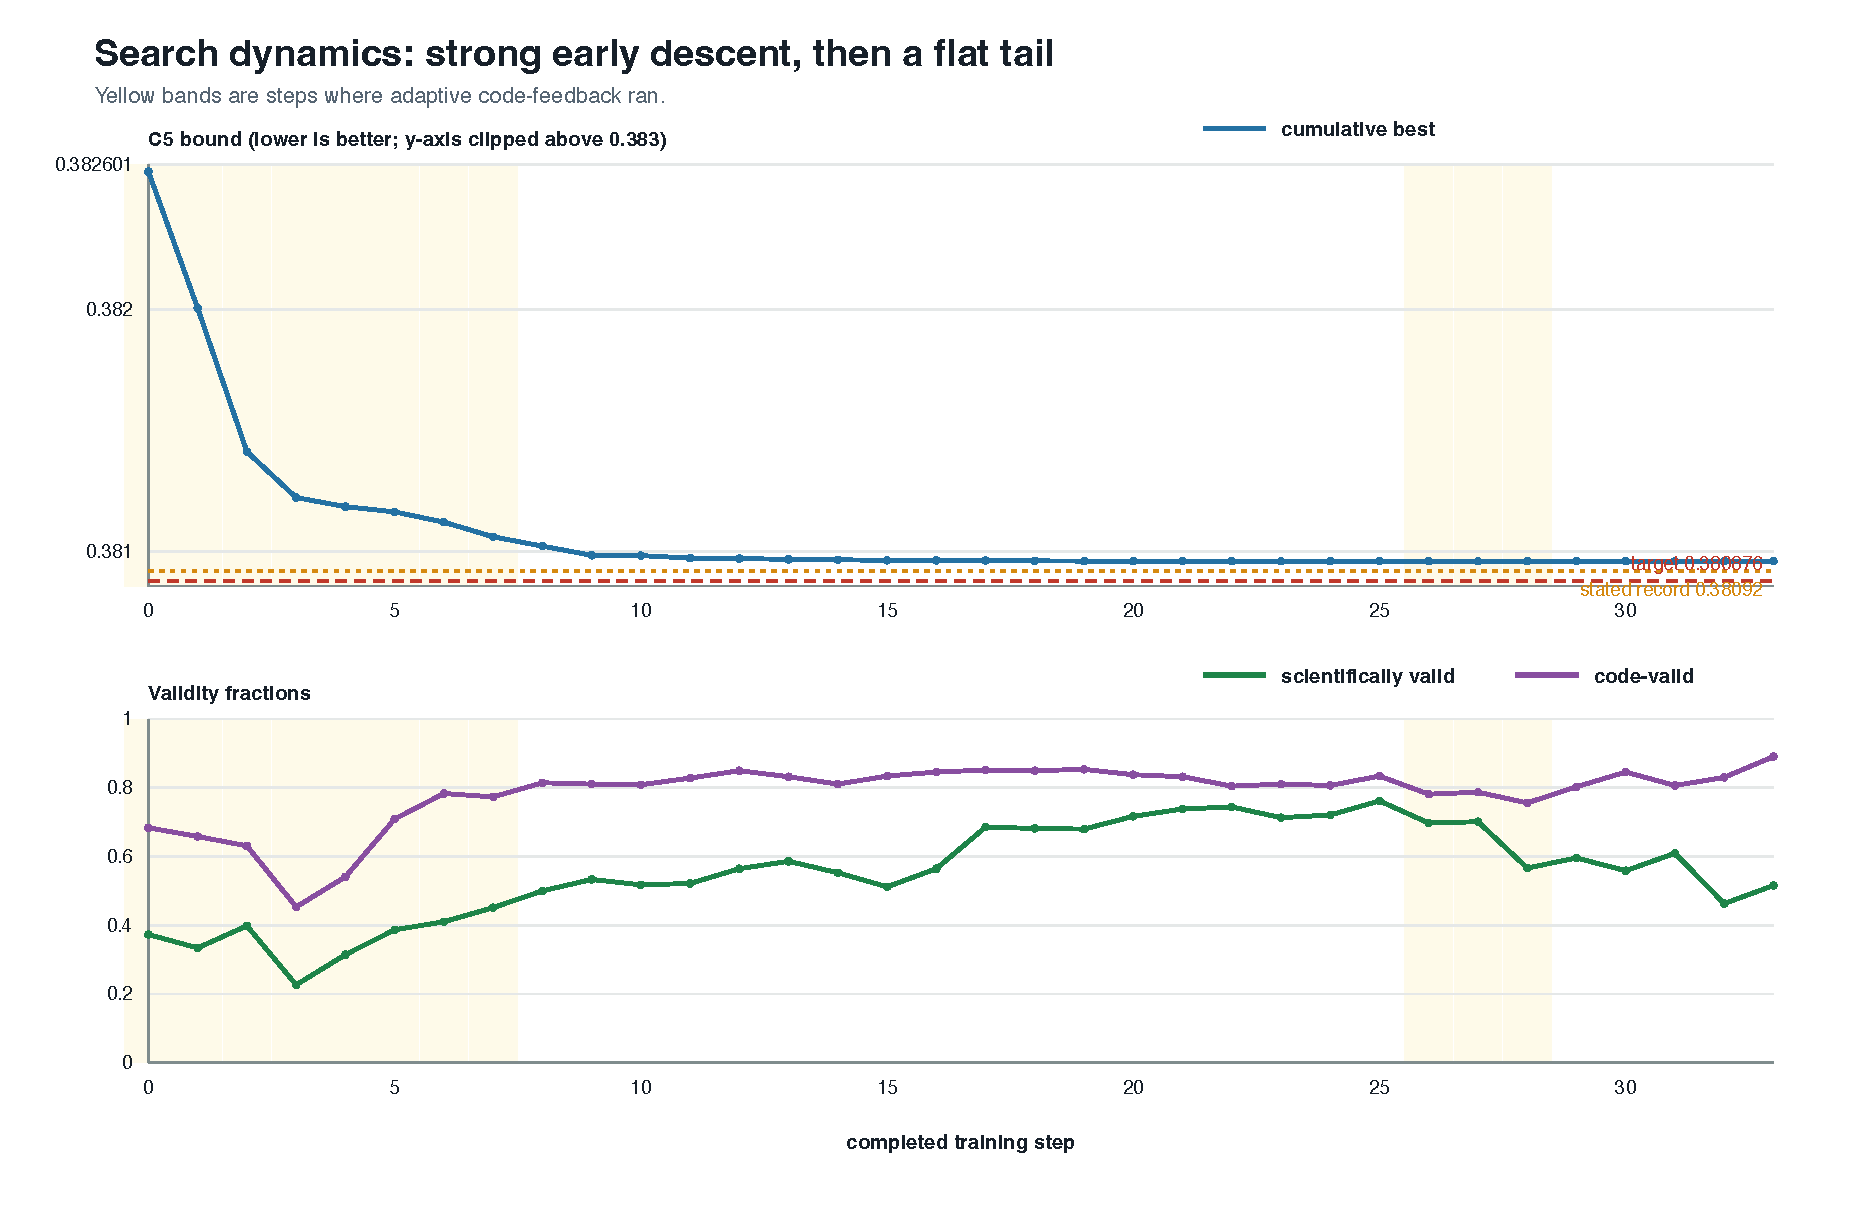
\includegraphics[width=0.96\textwidth]{figures/run_dynamics.pdf}
\caption{Search dynamics across the completed run. The incumbent improves rapidly and then reaches a long plateau, while code validity and scientific validity separate late in training. Yellow bands mark steps in which code-failure feedback was active.}
\label{figdynamics}
\end{figure*}

\begin{figure*}[t]
\centering
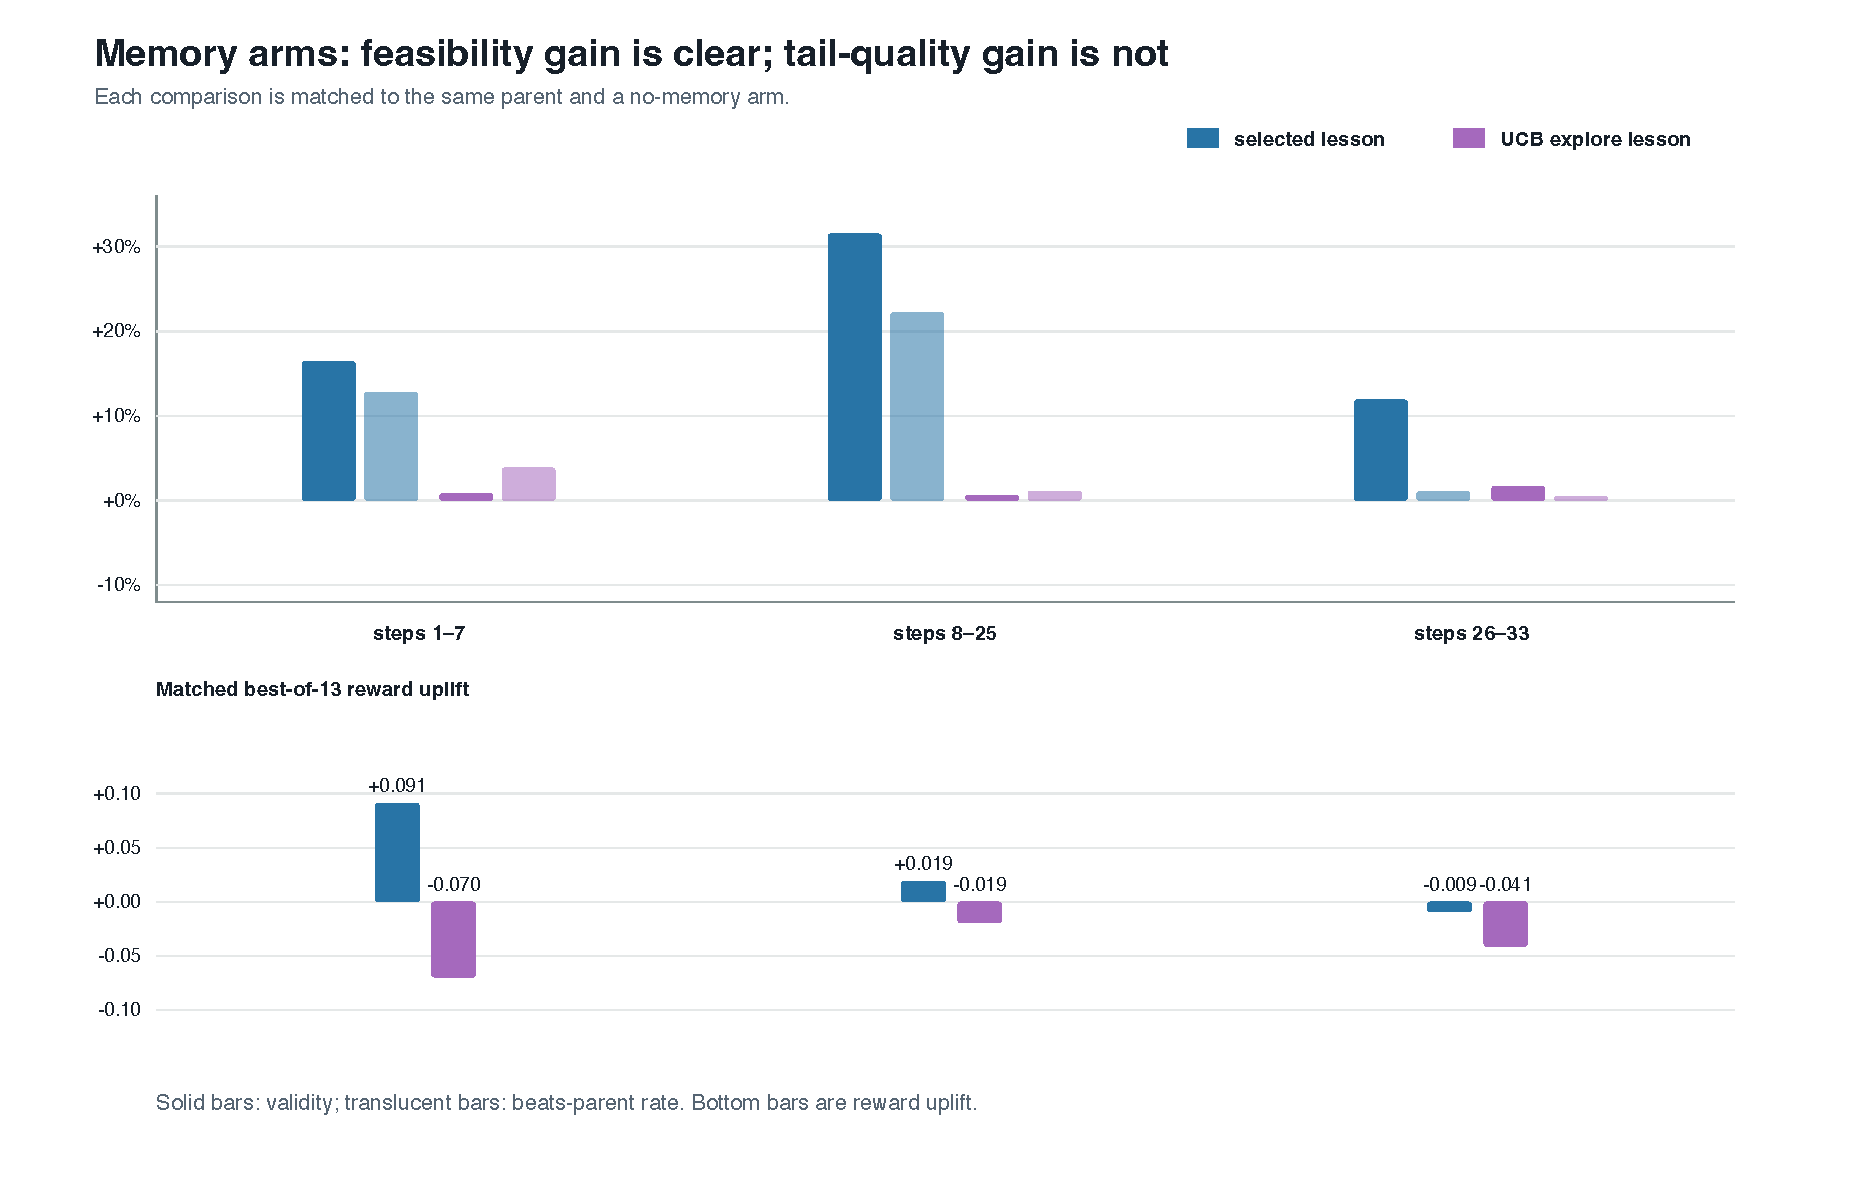
\includegraphics[width=0.96\textwidth]{figures/memory_effects.pdf}
\caption{Matched memory-arm comparisons. Selected memory consistently improves feasibility relative to the no-memory arm, but neither memory arm maintains a positive late reward-tail effect.}
\label{figmemoryeffects}
\end{figure*}

\begin{figure*}[t]
\centering
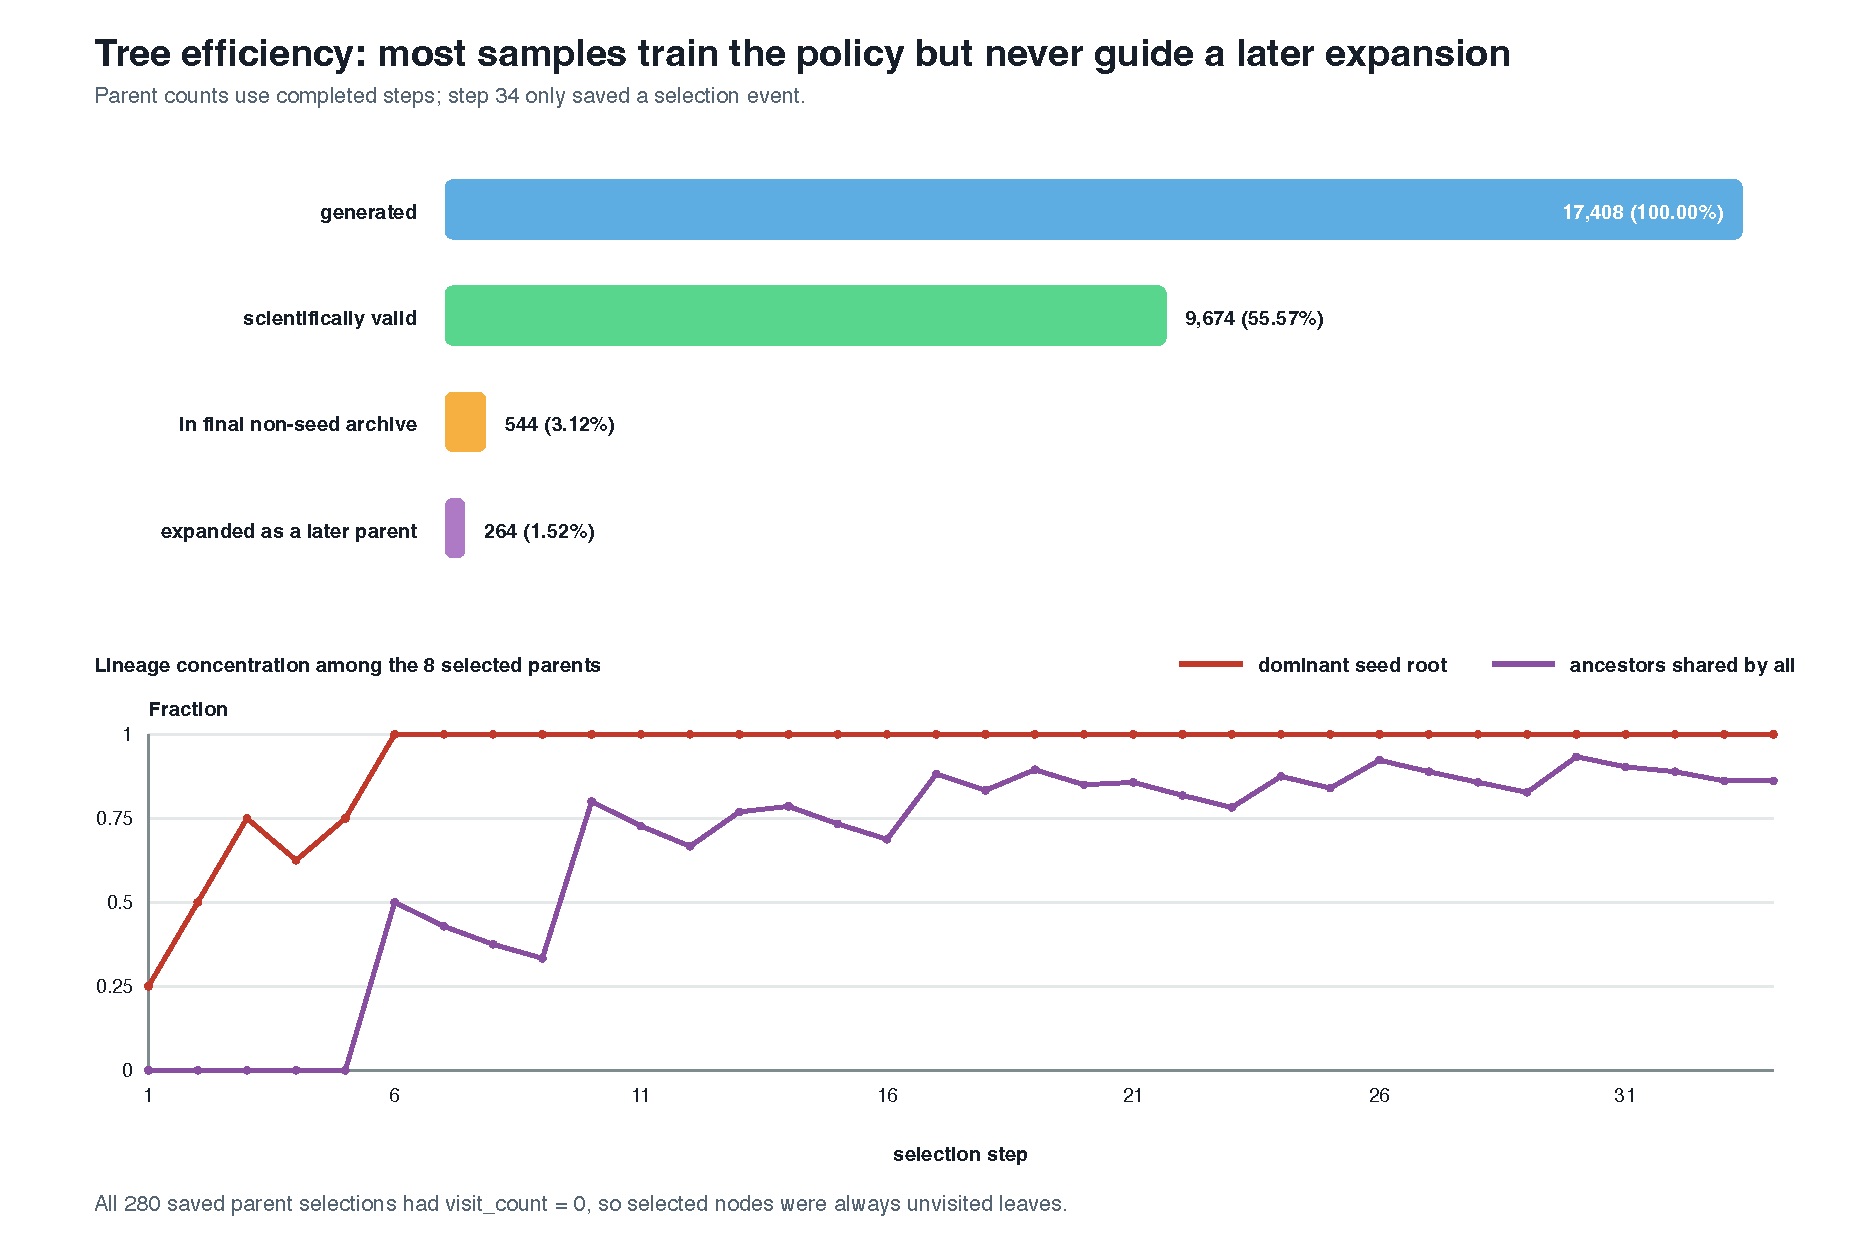
\includegraphics[width=0.96\textwidth]{figures/tree_efficiency.pdf}
\caption{Search-tree utilization and lineage concentration. Few generated candidates become later parents, and the active parent set rapidly concentrates on one seed lineage despite continued textual diversity.}
\label{figtreeefficiency}
\end{figure*}

\begin{table*}[t]
\centering
\small
\setlength{\tabcolsep}{5pt}
\begin{tabular}{@{}>{\raggedright\arraybackslash}p{0.17\textwidth}>{\raggedright\arraybackslash}p{0.35\textwidth}>{\raggedright\arraybackslash}p{0.42\textwidth}@{}}
\toprule
Component & Observation & Interpretation \\
\midrule
End-to-end search & Strong early descent followed by a stable plateau & The method finds a productive basin but does not keep opening new ones. \\
Memory & Higher feasibility under selected memory, without a robust late tail gain & Feasibility and scientific novelty require separate, recency-sensitive credit. \\
Code feedback & The adaptive controller and caps operated; no feedback-off control was present & Implementation is verified, but causal effectiveness remains unresolved. \\
Tree allocation & Fresh descendants dominated selection and the active roots collapsed & Visits and max backups did not progressively redirect the rollout budget. \\
Online learning & Late valid programs converged to the same construction and reward & The learning signal reduced to feasible versus infeasible rather than better versus worse science. \\
\bottomrule
\end{tabular}
\caption{Qualitative diagnosis of the analyzed run.}
\label{tabdiagnosis}
\end{table*}

\end{document}
